
\documentclass[xcolor=x11names,compress,10pt,handout]{beamer}

%% Beamer Layout %%%%%%%%%%%%%%%%%%%%%%%%%%%%%%%%%%
\useoutertheme[subsection=false,shadow]{miniframes}
\useinnertheme{default}
\usefonttheme{serif}
%\usepackage{palatino}

\usepackage{listings}
\usepackage{courier}
\lstset{basicstyle=\footnotesize\ttfamily,breaklines=true}
\lstset{
  backgroundcolor=\color{white!90!blue},
  basicstyle=\footnotesize\tt,     % the size of the fonts that are used for the code
  breakatwhitespace=false,         % sets if automatic breaks should only happen at whitespace
  breaklines=true,                 % sets automatic line breaking
  captionpos=b,                    % sets the caption-position to bottom
  extendedchars=true,              % lets you use non-ASCII characters; for 8-bits encodings only, does not work with UTF-8
  frame=single,                    % adds a frame around the code
  keywordstyle=\bf,
  showspaces=false,                % show spaces everywhere adding particular underscores; it overrides 'showstringspaces'
  showstringspaces=false,          % underline spaces within strings only
  showtabs=false,                  % show tabs within strings adding particular underscores
  tabsize=2                        % sets default tabsize to 2 spaces
}

\setbeamercolor*{lower separation line head}{bg=Firebrick4} 
\setbeamercolor*{normal text}{fg=black,bg=white} 
\setbeamercolor*{alerted text}{fg=red} 
\setbeamercolor*{example text}{fg=black} 
\setbeamercolor*{structure}{fg=Firebrick4} 
 
\setbeamercolor*{palette tertiary}{fg=black,bg=black!10} 
\setbeamercolor*{palette quaternary}{fg=black,bg=black!10} 

\renewcommand{\(}{\begin{columns}}
\renewcommand{\)}{\end{columns}}
\newcommand{\<}[1]{\begin{column}{#1}}
\renewcommand{\>}{\end{column}}


\newenvironment<>{block1}[1]{%
  \setbeamercolor{block title}{fg=black,bg=Firebrick4!15!white}%
  \begin{block}#2{#1}}{\end{block}}
  
  
\newenvironment<>{block2}[1]{%
  \setbeamercolor{block title}{fg=white,bg=blue!75!black}%
  \begin{block}#2{#1}}{\end{block}}

\newcommand{\by}{\mathbf{y}}
\newcommand{\bphi}{\boldsymbol{\phi}}

\setbeamercolor{block body}{fg=black,bg=gray!7}

\usepackage[absolute,overlay]{textpos}

% LOGO
\newcommand\FrameText[1]{%
  \begin{textblock*}{0.8\paperwidth}(40pt,.82\textheight)
    \raggedright #1\hspace{.5em}
  \end{textblock*}}
  
%\setbeamerfont{title like}{shape=\scshape}
\setbeamerfont{frametitle}{shape=\bf} 

\begin{document}


%%%%%%%%%%%%%%%%%%%%%%%%%%%%%%%%%%%%%%%%%%%%%%%%%%%%%%
%%%%%%%%%%%%%%%%%%%%%%%%%%%%%%%%%%%%%%%%%%%%%%%%%%%%%%
\begin{frame}
\title[]{\LARGE\bf\textcolor{black}{Introduction to network models}}
\subtitle[]{(Chapter 3 \& 4 of the manual)}
  
\author[]{\large\textcolor{Firebrick4}{\bf Alberto Caimo}\\ 
          }

\institute[]
  {\sc\normalsize Dublin Institute of Technology\\
   Ireland}

\date[]
  {}

\titlepage
 
 \FrameText{ \centering
 
\includegraphics[width=.8\textwidth]{ssnar_logo_slides}}

\end{frame}


%%
%\begin{frame}{Outline}
%\tableofcontents
%\end{frame}

%%
% \begin{itemize}
% \item
% \end{itemize}

% PART 1
\begin{frame}[fragile]{} 
\begin{center}
{\LARGE \bf Networks as random graphs} 
\end{center}
\end{frame}

%
\begin{frame}[fragile]{Networks as random graphs} 

\begin{block1}{\bf Definitions and notation}
\begin{itemize}
\item Networks are generally represented by graphs of nodes (actors) and edges (relations)
\item $N$ number of nodes (fixed).
\item $D$ number of dyads (pair of nodes) in a $N$-node network (fixed). 
\item $Y$ random $N \times N$ adjacency matrix where: 
 \begin{itemize}
 \item $Y_{ij} = 0$, if $i$ and $j$ are not connected; 
 \item $Y_{ij} = 1$, if $i$ and $j$ are connected;
 \item $Y_{ii} = 0$, (self-loops are not allowed).
 \end{itemize}
\item $y$ realisation of $Y$ (observed adjacency matrix);
\item $E = s_1(y)$ number of edges in the network (= number of 1's in $y$).
\end{itemize}
\end{block1}  
\end{frame}

%
\begin{frame}[fragile]{Networks as random graphs} 

{\bf Example - Lazega network}:\\ corporate law partnership in a Northeastern US corporate law firm
\begin{lstlisting}
library(statnet) 
load(url("https://acaimo.github.io/lazega.RData")) 
y <- network(Y, directed = FALSE)
set.seed(11) 
plot(y,
     vertex.col = "skyblue",
     vertex.cex = 2)
\end{lstlisting}
\end{frame}

%
\begin{frame}[fragile]{Networks as random graphs} 
\begin{center}
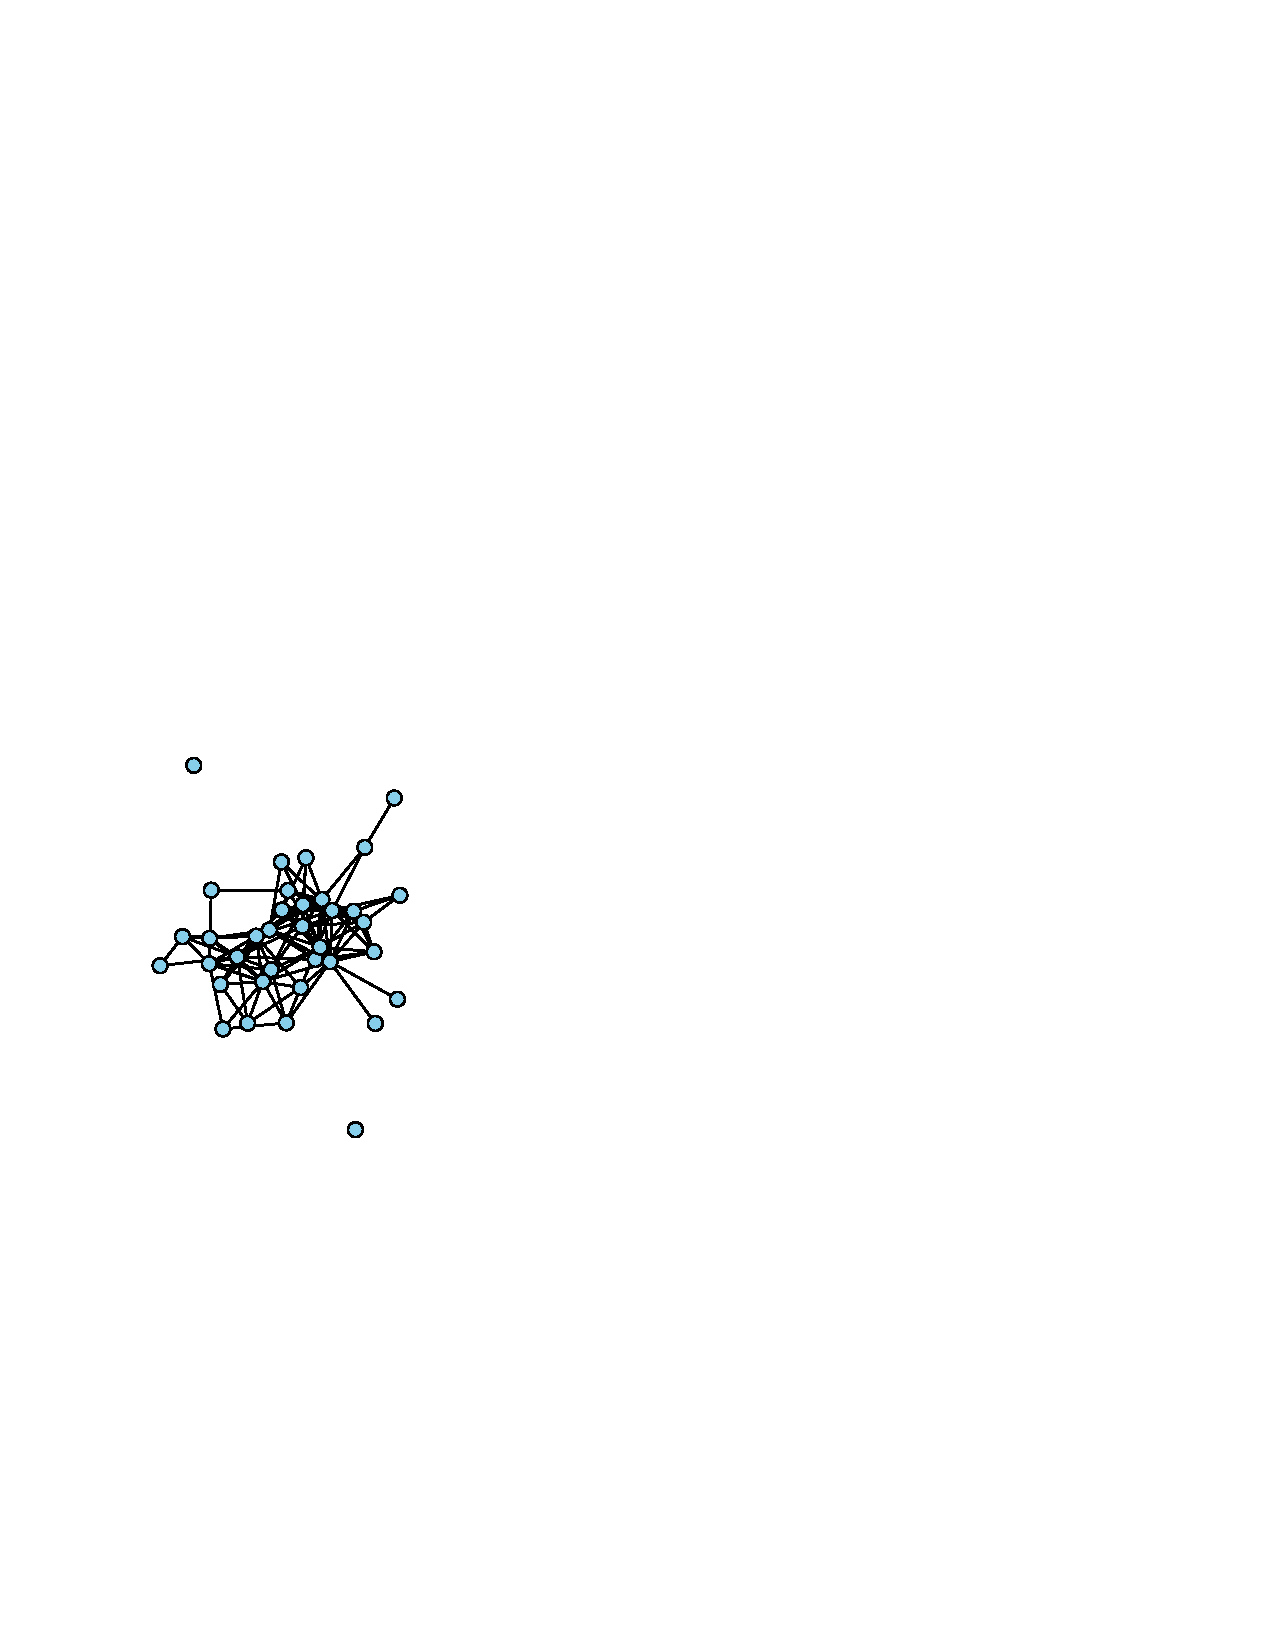
\includegraphics[scale=1]{lazega_graph}\\
{\bf Basic info}: undirected network, 36 nodes (partners and associates of the firm), 115 edges (co-work relations).
\end{center}
\end{frame}

%
\begin{frame}[fragile]{Networks as random graphs} 
Let's calculate some other descriptives:
\begin{itemize}
\item We know that $N = 36$;
\item What about the number of dyads $D$?\\ 
In an undirected graph, we have:
$$
D = \frac{N^2 - N}{2} = \frac{36^2 - 36}{2} = 630;
$$
\item In the Lazega network there are 115 edges, so $s_1(y) = 115$:
\begin{lstlisting}
s1 <- summary(y ~ edges); s1
\end{lstlisting}
\item Let's calculate the density of the network, i.e., the proportion of connected dyads:
$$
density(y) = \frac{s_1(y)}{D} = \frac{115}{630} \approx 0.1825 \approx 18.25\%.
$$
\end{itemize}
\end{frame}

%
\begin{frame}[fragile]{The random graph model} 
\begin{block1}{\bf Definition of the model}
$$
\Pr(Y = y) = \eta^{s_1(y)} (1 - \eta)^{D - s_1(y)}.
$$
\end{block1}
\begin{itemize}
\item Describe the probability of observing $y$ as a function of the parameter $\eta$;
\item The parameter $\eta$ represents the probability of observing an edge between any dyad;
\item To estimate the model we just need to estimate $\eta$:
$$
\hat{\eta} = \frac{s_1(y)}{D}.
$$ 
\item The parameter $\eta$ corresponds to the {\bf density} of the network.
\end{itemize}
\end{frame}

%
\begin{frame}[fragile]{The random graph model} 
\begin{block1}{\bf Definition of the model -- natural parametrisation}
$$
\Pr(Y = y) = \frac{\exp\{\theta s_1(y)\}}{c(\theta)}.
$$
\end{block1}
\begin{itemize}
\item The parameter $\theta$ is defined as the {\bf logit} of $\eta$:
$$
\theta = \log \left( \frac{\eta}{1-\eta} \right);
$$
\item $c(\theta)$ is a normalising constant;
\item The random graph model belongs to the {\bf exponential family} of models.
\end{itemize}
\end{frame}

%
\begin{frame}[fragile]{The random graph model} 

{\bf Parameter interpretation:}
\begin{itemize}
\item $\theta = 0 \Rightarrow \eta = 0.5$ (50\% of the dyads are not connected):
$$
\Pr(Y_{ij} = 1 | \theta = 0) = \frac{\exp\{0\}}{1 + \exp\{0\}} = \frac{1}{1 + 1} = \eta = 0.5.
$$
\item $\theta < 0 \Rightarrow \eta < 0.5$ (most of the dyads are not connected);
\item $\theta > 0 \Rightarrow \eta > 0.5$ (most of the dyads are connected).
\end{itemize}
\vspace{1cm}
Estimation of $\theta$ using {\bf statnet}:
\begin{lstlisting}
RG.model <- y ~ edges
theta <- ergm(RG.model)$coef
theta
\end{lstlisting}
\end{frame}

%
\begin{frame}[fragile]{Network simulation} 
To simulate from the estimated random graph model: 
\begin{itemize}
\item We can simply simulate $D$ Bernoulli trials by assuming $Y_{ij} \sim Bernoulli(\eta)$; 
\item Then we arrange them into a $N \times N$ matrix:
\end{itemize}
\vspace{.5cm}
\begin{lstlisting}
y.sim.1 <- simulate(RG.model, 
                    coef = theta)
plot(y.sim.1, 
     vertex.cex = 2, 
     vertex.col = 'skyblue', 
     main = 'y.sim.1')
\end{lstlisting}
\end{frame}

%
\begin{frame}[fragile]{Network simulation} 

Suppose that:
\begin{itemize}
\item We simulate 50 networks $\tilde{y} = \{ \tilde{y}_{1}, \tilde{y}_{2}, \dots, \tilde{y}_{50}\}$ from the estimated model;
\item $s_1(\tilde{y})$ is the vector containing the number of edges measured in each of the simulated networks; 
\item We calculate the average number of edges measured in the simulated networks as follows:
$$
E(s_1(\tilde{y})) = \frac{1}{M} \sum_{i = 1}^{M} s_1(\tilde{y_i});
$$
\item We expect that the average number of edges measured in the simulated networks is close to the observed number of edges in the observed network ($s_1(y)$): 
$$
E(s_1(\tilde{y})) \approx s_1(y).
$$
\end{itemize}
\end{frame}

%
\begin{frame}[fragile]{Network simulation} 
\begin{lstlisting}
y.sim.1_50 <- simulate(RG.model, 
                       coef = theta,
                       statsonly = TRUE, # returns only the 
                                         # network statistics 
                                         # in the model 
                                         # (number of edges)
                       nsim = 50) # number of network simulated

mean(y.sim.1_50) # ~115
\end{lstlisting}
\end{frame}

% PART 2
\begin{frame}[fragile]{} 
\begin{center}
{\LARGE \bf Exponential random graph models (ERGMs)} 
\end{center}
\end{frame}

%
\begin{frame}[fragile]{Basic assumptions} 

\begin{itemize}
\item The observed network $y$ is generated by a stochastic process in which edges are created because of the presence or absence of other edges (and possibly node-level attributes).
\item Local effects (represented by {\bf network statistics} $s(y)$) that generate dyadic relations and these processes may depend on the surrounding social environment.\\[.3cm]
\end{itemize} 

For example:
\begin{itemize}
\item We can assume that actors with similar attributes are more likely to form friendship edges ({\bf homophily});
\item If two unconnected actors were connected to a third actor, at some point they are likely to form a friendship link between them ({\bf transitivity}). 
\end{itemize}
\end{frame}

%
\begin{frame}[fragile]{Exponential random graph models} 
\begin{block1}{\bf Definition of the model}
Exponential family representing the probability distribution of $y$ given a vector of parameters $\theta$:
$$
\Pr(Y = y | \theta) = \frac{\exp\{\theta^T s(y)\}}{c(\theta)}.
$$
\end{block1}

\begin{itemize}
\item Describe the probability of observing $y$ as a function of the parameter $\theta$;
\item $s(y)$ is a vector of network statistics (e.g. number of edges, number of triangles, etc.) associated to effects of interest;
\item $\theta$ is the vector of parameters associated to the network statistics $s(y)$;
\item $c(\theta)$ is a normalising constant which \textcolor{red}{\bf cannot} be computed for not trivially small networks.
\end{itemize}
\end{frame}

%
\begin{frame}[fragile]{Dependence assumptions and network statistics} 
\begin{itemize}
\item Dyadic dependence (as in the random graph model) is an unrealistic assumption in many circumstances;
\item Network statistics involving more than a dyad imply {\bf dependence} between dyads: an edge between node $i$ and $j$ is assumed to be dependent on the presence of other edges.\\[.3cm]
\end{itemize}

For example:
\begin{itemize}
\item {\bf Stars} statistics assume that an edge between $i$ and $j$ is contingent on any possible edge involving node $i$ and $j$ (i.e. on the degrees of $i$ and $j$).
\item {\bf Triadic} statistics assume that an edge between $i$ and $j$ is contingent on any possible edge involving any node of the network connected to both $i$ and $j$.
\end{itemize}
\end{frame}

%
\begin{frame}[fragile]{Parameter interpretation} 
\begin{itemize}
\item The parameter $\theta$ associated with the network effects expressed by the network statistics $s(y)$ provide insights about the contribution of each network statistic to edge formation. 
\item ERGMs allow to establish a relationship between presence/absence of an edge and a set of network statistics.
\end{itemize}
\end{frame}

%
\begin{frame}[fragile]{Parameter interpretation} 
For example, suppose $s(y)$ includes the number of edges ($s_1(y)$) and the number of 2-stars ($s_2(y)$).
\begin{itemize}
\item $\theta_1 < 0 | \theta_2 \Rightarrow$ sparse network;
\item $\theta_1 > 0 | \theta_2 \Rightarrow$ dense network;
\item $\theta_2 > 0 | \theta_1 \Rightarrow$ edges tend to connect nodes with high degree (i.e. presence of high-degree nodes);
\item $\theta_2 < 0 | \theta_1 \Rightarrow$ absence of high-degree nodes;
\end{itemize}
\end{frame}

\end{document}